\usetikzlibrary{shapes.geometric, arrows}
\tikzstyle{startstop} = [ellipse, minimum width=2cm, minimum height=2cm, text centered, draw=black]
\tikzstyle{process} = [rectangle, minimum width=2cm, minimum height=2cm, text centered, draw=black]
\tikzstyle{decision} = [diamond, minimum width=2cm, minimum height=2cm, text centered, draw=black]
\tikzstyle{arrow} = [thick,->,>=stealth]

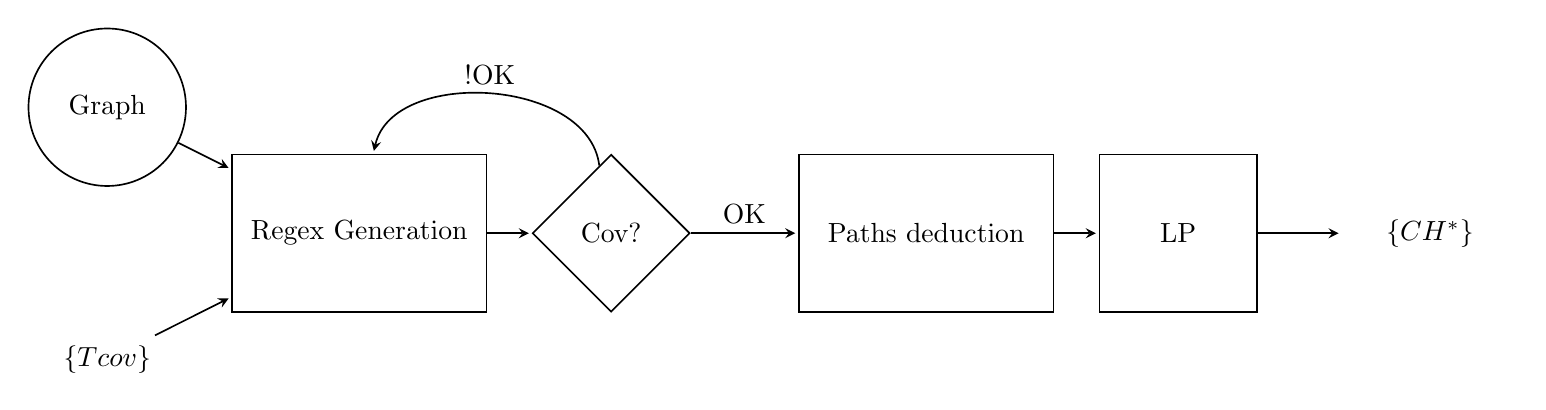
\begin{tikzpicture}[->,>=stealth,shorten >=1pt,auto,semithick,scale=0.8,node distance=2.5cm]

    % Nodes
    \node[startstop] (graph) at (0,2cm) {Graph};
    \node (tcov) at (0,-2cm) {$\{Tcov\}$};

    \node[process] (regExpGen) at (4cm, 0) {\makebox[3cm][c]{Regex Generation}};
    \node[decision] (covCheck) at (8cm, 0) {Cov?};
    \node[process] (pathsDeduction) at (13cm, 0) {\makebox[3cm][c]{Paths deduction}};
    \node[process] (lp) at (17cm, 0) {LP};
    \node (output) at (21cm, 0) {\makebox[2cm][c]{$\{CH^*\}$}};

    % Arrows
    \path
    (graph) edge[bend left=0, above] node {} (regExpGen)
    (tcov) edge[bend left=0, above] node {} (regExpGen)
    
    (regExpGen) edge[bend left=0, above] node {} (covCheck)
    (covCheck) edge[bend left=0, above] node {OK} (pathsDeduction)
    (pathsDeduction) edge[bend left=0, above] node {} (lp)
    (lp) edge[bend left=0, above] node {} (output)
    (covCheck) edge[bend right=80, above] node {!OK} (regExpGen);

\end{tikzpicture}
